\section{L'Homme gouverne l'Homme}

\paragraph{} Les hommes possèdent donc, aujourd'hui, \emph{toutes} les architectures et réseaux
nécessaires afin d'être mis en relation. L'échange de données, l'accès à des plateformes
\emph{centralisées}, sont \emph{instantanés}. Les notions de consommation et de production
sont maintenant intrinséquement liées : on ne peut plus \emph{consommer sans produire}, ni même
\emph{produire sans consommer}. L'Homme est devenu \emph{consommacteur} de technologies.

\paragraph{} À travers la mise en \oe{}uvre à grande échelle, l'Homme peut être
\emph{partout, tout le temps}. Il en découle un statut particulier de l'Homme 
technologique : producteur et consommateur \emph{intemporel}, l'Homme devient \emph{Omniscient}.
Il fait partie du \emph{Réseau}, parce qu'il est présent sur \emph{les réseaux}. Notre identité
est avant tout constituée des \emph{multiples briques d'identité} que nous acceptons de
\emph{partager}.

\paragraph{} Mais faire partie du réseau, n'est-ce pas déjà en soi \emph{y participer} ? L'\oe{}uvre
de Masamune Shirow, \emph{Ghost In the Shell} \cite{GhostInTheShell}, nous fournit l'enseignement
suivant : dans la société sur-technologisée, ce n'est plus \emph{l'action} qui détermine la
\emph{participation} - c'est \emph{l'existence}. Dès lors, si l'Homme souhaite se \emph{libérer}
des contraintes technologiques, il ne lui reste qu'une possibilité : \emph{ne pas exister} au
sein des réseaux.

\paragraph{} Que cela implique-t-il ? Selon nous, une \emph{autarcie complète}. Nous avons vu que la
collecte est maintenant \emph{insidieuse} : au-delà des réseaux, \emph{tout est collecté} (transports,
santé, citoyenneté) et ne permet même plus à l'Homme d'agir \emph{librement}, en respectant son
\emph{anonymat}. Pourtant même cette autarcie nous semble \emph{difficilement accessible}. Chaque foyer,
chaque personne, chaque entité forme un n\oe{}ud du réseau. La surveillance n'est pas automatique : 
elle se nourrit de nos interactions. C'est donc bien que nous devons \emph{cesser d'interagir} si nous
souhaitons échapper à la part de \emph{règles et de contrôle} que porte chacun : comme le précisait Sartre,
finalement, \guillemotleft L'enfer, c'est les autres\guillemotright \cite{Sartre0}.


\subsection*{Régulation, adoption}

\paragraph{} La surveillance naît de la crainte et des peurs de l'Homme, qui souhaite que les règles qu'il se fixe 
s'appliquent à tous. On constate ainsi une volonté constante des États de \emph{réguler} l'usage des innovations technologiques
disruptives. Mais cela ne fait souvent que souligner le fait qu'ils sont totalement dépassés par certaines de ces 
avancées technologiques. Toutes les technologies doivent-elles être régulées, contrôlées par un organe étatique ? Deux 
exemples opposés s'offrent à nous. 

\paragraph{} D'un côté, en France, le téléchargement sur des réseaux \emph{peer-to-peer} est surveillé et "contrôlé" 
dans le cas des \oe{}uvres protégées par le droit de propriété intellectuelle. Cependant, cette régulation n'est qu'indirecte :
en effet, il est impossible d'empêcher le téléchargement d'un flux de données sous prétexte que ces informations \emph{précises}
tombent sous le coup d'une juridiction qui n'a aucune forme de matérialité au sein du réseau. Ainsi, dans le cas de la
\emph{Hadopi} (\emph{Haute Autorité pour la Diffusion des \OE{}uvres et la Protection des droits sur Internet}), les sanctions
encourues par les contrevenants ne relèvent pas de la \emph{contrefaçon} - dénomination légale s'appliquant à la copie d'une
\oe{}uvre protégée - mais de la \emph{négligence caractérisée}, le contrevenant ayant alors tardé à \emph{sécuriser son
réseau} pour empêcher ledit téléchargement. Cette subtilité légale n'est pas due à une incompétence ou une incompréhension
quelconque du fonctionnement de ces technologies - bien au contraire. C'est un aveu d'échec, d'impuissance face au fonctionnement
même de ces technologies.

\paragraph{} Un autre exemple est celui des cryptomonnaies, qui tardent à être régulées à travers le monde. Dans ce cas
précis ce sont les \emph{exchanges}, pivot des transactions entre monnaie numérique et monnaie fiduciaire, qui sont le 
plus souvent impactés par les sautes d'humeur gouvernementales. La technologie en elle-même est restée jusque-là irrégulée,
bien que les bénéfices effectués sur ces réseaux doivent malgré tout être déclarés. Un exemple particulier est celui des 
États-Unis, qui considèrent les cryptomonnaies à l'identique des \emph{stock-options} d'un point de vue fiscal. Ainsi, 
là où en France seuls les bénéfices effectués suite à la reconversion en euros doivent être déclarés en BNC (bénéfices non
commerciaux), aux États-Unis le simple fait d'échanger une valeur de cryptomonnaie pour une autre (acheter 0.1 BTC pour 
1 ETH, par exemple) est une action qui doit être déclarée à l'administration fiscale.

\paragraph{} Quels enseignements peut-on alors tirer des gouvernements qui essaient, eux, d'\emph{adopter} ces technologies ? 
Nous pouvons ici prendre l'exemple de l'\emph{e-nationalité} estonienne dans la blockchain \cite{Blockchain3}. Cela permet
à n'importe quel individu d'obtenir une \emph{nationalité estonienne numérique} qui, si elle n'a pas valeur légale de
nationalité estonienne à proprement parler, délivre tout de même à la personne des documents d'identité et la possibilité
de démarrer une activité économique au sein de l'Union Européenne.

\begin{figure}[ht]
    \centering
    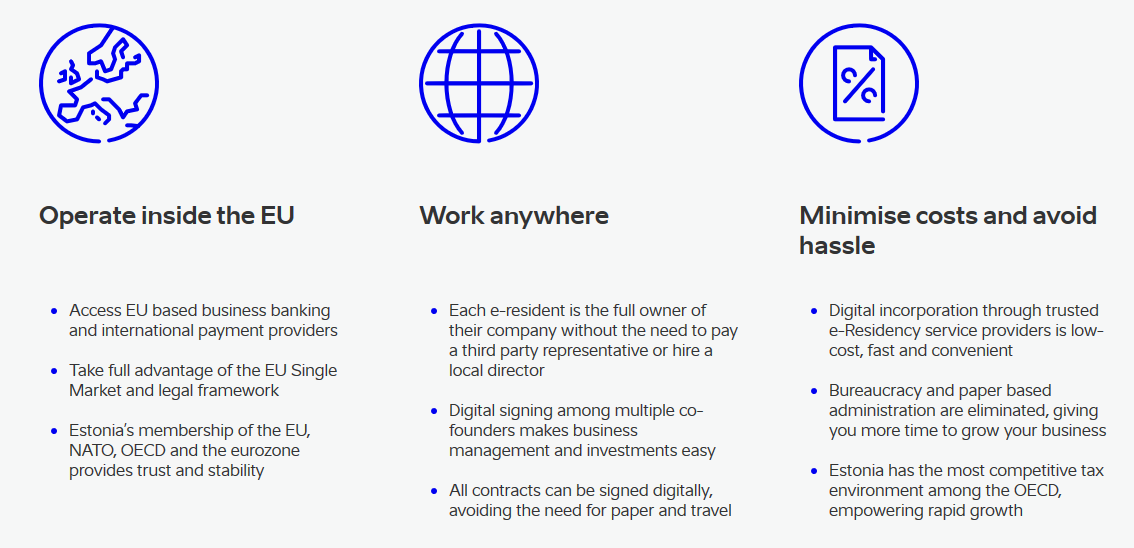
\includegraphics[width=400px]{chapters/02/images/eresidency.png}
    \caption{\label{eresidency}Les avantages à démarrer une activité économique en tant qu'\emph{e-résident} estonien.}
\end{figure}

\paragraph{} Finalement, le programme d'e-nationalité entamé par l'Estonie est une démarche extrêmement maligne. Plutôt
que de se \emph{confronter} à une technologie mal comprise par de nombreux gouvernements, l'Estonie a pris le partie de
l'\emph{embrasser} pour en tirer profit. En effet, il n'est pas à douter que les entreprises qui verront le jour à travers
ce programme participeront à l'essor économique du pays.

\subsection*{Neutralité, égalité}

\paragraph{} Une question récente de régulation des réseaux est celle de \emph{la neutralité du Net},
beaucoup discutée aux États-Unis depuis 2015 et l'arrivée du nouveau président américain. Le 14 décembre
dernier, suite à ces évènements, les États-Unis abrogeaient ce principe fondateur d'Internet \cite{NetNeutrality0}.
Désormais, tous les contenus mis en ligne n'ont pas obligation à être traités de la même manière par
les fournisseurs d'accès internet. Ces derniers peuvent donc choisir de ralentir ou d'accélérer la communication
avec un site donné.

\begin{figure}[ht]
    \centering
    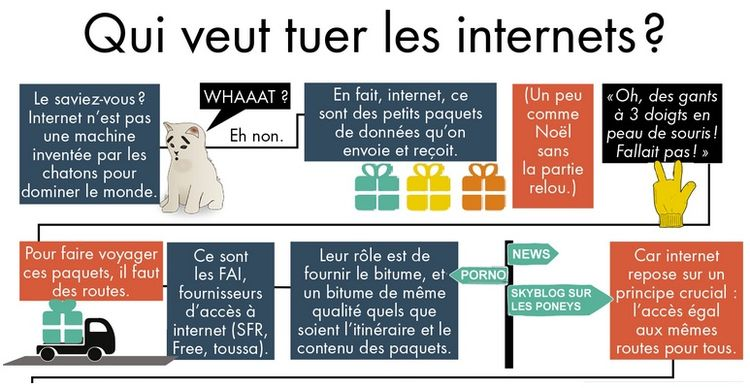
\includegraphics[width=350px]{chapters/02/images/internet_cats.jpg}
    \caption{\label{netneutrality}La neutralité du Net \cite{NetNeutrality1}.}
\end{figure}

\paragraph{} Cette forme \emph{d'inégalité} est dangereuse car elle met en péril les fondements même d'Internet
en en faisant une plateforme avant tout commerciale. Cela oblige certains utilisateurs à modifier leurs habitudes 
d'utilisation et les invite à trouver des moyens détournés - en passant par les \emph{réseaux parallèles} par exemple -
pour parvenir à conserver leurs usages d'origine. En France, la neutralité du Net à été estimée comme étant un \emph{droit} 
par le \emph{Conseil Constitutionnel}, ce qui constitue selon nous une avancée importante. En reconnaissant la
nécessité de pouvoir s'exprimer librement et d'avoir accès de manière égale aux différents contenus proposés
sur Internet, le gouvernement s'inscrit dans une relation de confiance avec la population qui nous semble
nécessaire dans le contexte géopolitique actuel. Nombreux sont les pays dans lesquels l'accès à Internet
est contrôlé. Gouvernement religieux, autocratique, totalitaire, militariste... Chaque contexte implique
des restrictions différentes, mais qui portent atteinte selon nous à \emph{la liberté d'expression}.

\paragraph{} Remarquons que les \emph{cryptomonnaies} sont particulièrement sensibles aux \emph{comportements
et annonces} des différents gouvernements vis-à-vis de cette technologie. Ainsi, courant janvier 2018, le Bitcoin
ainsi que différentes cryptomonnaies perdaient jusqu'à plus de 20\% de leur valeur suite à l'annonce par un membre du
gouvernement corréen que \emph{l'accès aux plateformes d'échanges seraient interdit} dans le pays
- annonce qui sera réfutée plus tard par le gouvernement \cite{CryptoMonnaies0}. Quelques mois avant, en septembre 2017, 
c'était une annonce d'une grande plateforme chinoise d'échange qui faisait perdre au Bitcoin 17\% de sa valeur en deux 
jours \cite{CryptoMonnaies1}.

\paragraph{} Finalement, Internet et les réseaux à grande échelle restent - bien qu'indirectement - contrôlés par des 
entités gouvernementales et politiques. Les fournisseurs d'accès Internet et les hébergeurs sont devenus deux 
nouvelles puissances actives \emph{d'établissement ou de relâchement du contrôle}. Les utilisateurs quant à eux
acceptent \emph{davantage} de contrôle et ce plus \emph{facilement} qu'auparavant. L'accès à des données personnelles
n'est pas questionné car il n'est parfois même pas \emph{conscient}.